% Options for packages loaded elsewhere
% Options for packages loaded elsewhere
\PassOptionsToPackage{unicode}{hyperref}
\PassOptionsToPackage{hyphens}{url}
\PassOptionsToPackage{dvipsnames,svgnames,x11names}{xcolor}
%
\documentclass[
  11pt,
]{article}
\usepackage{xcolor}
\usepackage[margin=1in]{geometry}
\usepackage{amsmath,amssymb}
\setcounter{secnumdepth}{5}
\usepackage{iftex}
\ifPDFTeX
  \usepackage[T1]{fontenc}
  \usepackage[utf8]{inputenc}
  \usepackage{textcomp} % provide euro and other symbols
\else % if luatex or xetex
  \usepackage{unicode-math} % this also loads fontspec
  \defaultfontfeatures{Scale=MatchLowercase}
  \defaultfontfeatures[\rmfamily]{Ligatures=TeX,Scale=1}
\fi
\usepackage{lmodern}
\ifPDFTeX\else
  % xetex/luatex font selection
\fi
% Use upquote if available, for straight quotes in verbatim environments
\IfFileExists{upquote.sty}{\usepackage{upquote}}{}
\IfFileExists{microtype.sty}{% use microtype if available
  \usepackage[]{microtype}
  \UseMicrotypeSet[protrusion]{basicmath} % disable protrusion for tt fonts
}{}
\makeatletter
\@ifundefined{KOMAClassName}{% if non-KOMA class
  \IfFileExists{parskip.sty}{%
    \usepackage{parskip}
  }{% else
    \setlength{\parindent}{0pt}
    \setlength{\parskip}{6pt plus 2pt minus 1pt}}
}{% if KOMA class
  \KOMAoptions{parskip=half}}
\makeatother
% Make \paragraph and \subparagraph free-standing
\makeatletter
\ifx\paragraph\undefined\else
  \let\oldparagraph\paragraph
  \renewcommand{\paragraph}{
    \@ifstar
      \xxxParagraphStar
      \xxxParagraphNoStar
  }
  \newcommand{\xxxParagraphStar}[1]{\oldparagraph*{#1}\mbox{}}
  \newcommand{\xxxParagraphNoStar}[1]{\oldparagraph{#1}\mbox{}}
\fi
\ifx\subparagraph\undefined\else
  \let\oldsubparagraph\subparagraph
  \renewcommand{\subparagraph}{
    \@ifstar
      \xxxSubParagraphStar
      \xxxSubParagraphNoStar
  }
  \newcommand{\xxxSubParagraphStar}[1]{\oldsubparagraph*{#1}\mbox{}}
  \newcommand{\xxxSubParagraphNoStar}[1]{\oldsubparagraph{#1}\mbox{}}
\fi
\makeatother


\usepackage{longtable,booktabs,array}
\usepackage{calc} % for calculating minipage widths
% Correct order of tables after \paragraph or \subparagraph
\usepackage{etoolbox}
\makeatletter
\patchcmd\longtable{\par}{\if@noskipsec\mbox{}\fi\par}{}{}
\makeatother
% Allow footnotes in longtable head/foot
\IfFileExists{footnotehyper.sty}{\usepackage{footnotehyper}}{\usepackage{footnote}}
\makesavenoteenv{longtable}
\usepackage{graphicx}
\makeatletter
\newsavebox\pandoc@box
\newcommand*\pandocbounded[1]{% scales image to fit in text height/width
  \sbox\pandoc@box{#1}%
  \Gscale@div\@tempa{\textheight}{\dimexpr\ht\pandoc@box+\dp\pandoc@box\relax}%
  \Gscale@div\@tempb{\linewidth}{\wd\pandoc@box}%
  \ifdim\@tempb\p@<\@tempa\p@\let\@tempa\@tempb\fi% select the smaller of both
  \ifdim\@tempa\p@<\p@\scalebox{\@tempa}{\usebox\pandoc@box}%
  \else\usebox{\pandoc@box}%
  \fi%
}
% Set default figure placement to htbp
\def\fps@figure{htbp}
\makeatother


% definitions for citeproc citations
\NewDocumentCommand\citeproctext{}{}
\NewDocumentCommand\citeproc{mm}{%
  \begingroup\def\citeproctext{#2}\cite{#1}\endgroup}
\makeatletter
 % allow citations to break across lines
 \let\@cite@ofmt\@firstofone
 % avoid brackets around text for \cite:
 \def\@biblabel#1{}
 \def\@cite#1#2{{#1\if@tempswa , #2\fi}}
\makeatother
\newlength{\cslhangindent}
\setlength{\cslhangindent}{1.5em}
\newlength{\csllabelwidth}
\setlength{\csllabelwidth}{3em}
\newenvironment{CSLReferences}[2] % #1 hanging-indent, #2 entry-spacing
 {\begin{list}{}{%
  \setlength{\itemindent}{0pt}
  \setlength{\leftmargin}{0pt}
  \setlength{\parsep}{0pt}
  % turn on hanging indent if param 1 is 1
  \ifodd #1
   \setlength{\leftmargin}{\cslhangindent}
   \setlength{\itemindent}{-1\cslhangindent}
  \fi
  % set entry spacing
  \setlength{\itemsep}{#2\baselineskip}}}
 {\end{list}}
\usepackage{calc}
\newcommand{\CSLBlock}[1]{\hfill\break\parbox[t]{\linewidth}{\strut\ignorespaces#1\strut}}
\newcommand{\CSLLeftMargin}[1]{\parbox[t]{\csllabelwidth}{\strut#1\strut}}
\newcommand{\CSLRightInline}[1]{\parbox[t]{\linewidth - \csllabelwidth}{\strut#1\strut}}
\newcommand{\CSLIndent}[1]{\hspace{\cslhangindent}#1}



\setlength{\emergencystretch}{3em} % prevent overfull lines

\providecommand{\tightlist}{%
  \setlength{\itemsep}{0pt}\setlength{\parskip}{0pt}}



 


\makeatletter
\@ifpackageloaded{caption}{}{\usepackage{caption}}
\AtBeginDocument{%
\ifdefined\contentsname
  \renewcommand*\contentsname{Table of contents}
\else
  \newcommand\contentsname{Table of contents}
\fi
\ifdefined\listfigurename
  \renewcommand*\listfigurename{List of Figures}
\else
  \newcommand\listfigurename{List of Figures}
\fi
\ifdefined\listtablename
  \renewcommand*\listtablename{List of Tables}
\else
  \newcommand\listtablename{List of Tables}
\fi
\ifdefined\figurename
  \renewcommand*\figurename{Figure}
\else
  \newcommand\figurename{Figure}
\fi
\ifdefined\tablename
  \renewcommand*\tablename{Table}
\else
  \newcommand\tablename{Table}
\fi
}
\@ifpackageloaded{float}{}{\usepackage{float}}
\floatstyle{ruled}
\@ifundefined{c@chapter}{\newfloat{codelisting}{h}{lop}}{\newfloat{codelisting}{h}{lop}[chapter]}
\floatname{codelisting}{Listing}
\newcommand*\listoflistings{\listof{codelisting}{List of Listings}}
\makeatother
\makeatletter
\makeatother
\makeatletter
\@ifpackageloaded{caption}{}{\usepackage{caption}}
\@ifpackageloaded{subcaption}{}{\usepackage{subcaption}}
\makeatother
\usepackage{bookmark}
\IfFileExists{xurl.sty}{\usepackage{xurl}}{} % add URL line breaks if available
\urlstyle{same}
\hypersetup{
  pdftitle={Courier Assignment and Bottleneck Detection in Urban Food Delivery: Network Structure and Operational Capacity in Washington, DC},
  pdfauthor={Bryce Grover; Tianyu Zhao},
  colorlinks=true,
  linkcolor={blue},
  filecolor={Maroon},
  citecolor={Blue},
  urlcolor={Blue},
  pdfcreator={LaTeX via pandoc}}


\title{Courier Assignment and Bottleneck Detection in Urban Food
Delivery: Network Structure and Operational Capacity in Washington, DC}
\author{Bryce Grover \and Tianyu Zhao}
\date{2026-08-05}
\begin{document}
\maketitle
\begin{abstract}
Food delivery in a city depends on the road network underneath it. We
study Washington, DC using the OpenStreetMap drivable network, 2,043
restaurant locations, census tract population as a demand proxy,
observed 2024 traffic counts, and a simulated day of 15,188 orders.
Travel time weighted betweenness finds a short list of chokepoints led
by the 3rd Street Tunnel and the Southeast Freeway, and simple metrics
like observed volume or speed miss most of them. Restaurants cluster
strongly (Clark-Evans R of 0.32) and clustered restaurants reach demand
about 16 percent faster than isolated ones. Upgrading the most central
slow streets helps, but only at corridor scale. The demand ceiling is a
limit on orders per hour rather than on daily volume, near 1,500 orders
per hour for a 500 courier fleet, and it binds at dinner.
\end{abstract}


\section{Introduction}\label{introduction}

Nowadays, food delivery has become common in most cities. However,
customers usually only see the final delivery time. The process behind
each order is much more complex. The platform needs to assign a courier,
select a route, and deliver the order under changing traffic and demand
conditions.

Previous studies mainly focus on courier assignment and route
optimization. However, they pay less attention to how the road network
itself affects delivery performance. Even with a good assignment
strategy, important roads or intersections may still become bottlenecks.
Road closures and high demand can also cause longer delivery times.
Based on this, our project studies both the road network and courier
assignment strategies.

To start the analysis, we use the Washington, DC road network from
OpenStreetMap. We also use restaurant locations, population data, 2024
traffic counts, and a simulated day containing 15,188 orders. Also, the
population density is used to represent customer demand. The simulated
orders include lunch and dinner peaks, which allows us to test the
delivery system under different demand levels.

Our analysis contains two main parts. First, we examine the structure of
the road network. By applying bottleneck detection, estimating the
demand ceiling, testing renovation targets, and measuring the clustering
effect, we came up with 4 structural questions:

\begin{enumerate}
\def\labelenumi{\arabic{enumi}.}
\tightlist
\item
  \emph{RQ1.} Does a three-stage curriculum (quadrant, enumeration,
  diagnosis) improve DENTEX disease-detection performance over a
  single-stage baseline trained only on the fully labeled tier?
\item
  \emph{RQ2.} Which curriculum stage contributes most to the final
  model's performance?
\item
  \emph{RQ3.} How do realistic image degradations affect YOLOv8 disease
  detection performance, and does training with degraded images improve
  robustness?
\item
  \emph{RQ4.} To what extent does region-focused preprocessing improve
  YOLOv8 disease detection performance compared with using the full
  panoramic image?
\end{enumerate}

Then, we examine delivery operations by comparing two courier assignment
strategies. We also test their performance during peak hours, under road
closures, and with different fleet sizes, and then came up with 4
operational questions:

To sum up, this project studies how road structure and courier
assignment work together in an urban food delivery system. Based on the
results, we can better understand what causes delivery delays, which
roads are the most important, and how many couriers are needed for
reliable delivery performance.

\section{Data}\label{data}

The drivable street network for Washington, DC was downloaded from
OpenStreetMap with OSMnx. Cleaning kept the largest strongly connected
component, which leaves 10,027 intersections and 26,938 directed edges
(1,928 km of streets) and means every location can reach every other
along legal driving directions. Only about a third of edges have an
explicit speed tag, so missing speeds were filled in with the mean
tagged speed of the same road type, and every edge got a free flow
travel time weight. These free flow times ignore congestion, which is a
limitation that carries into every result below.

Restaurant POIs come from OpenStreetMap amenity tags for restaurants,
fast food, and cafes, which gives 2,043 locations after removing same
name duplicates within 50 m. Each POI was snapped to the network with a
median snap distance of 19.4 m. As an outside check on coverage, 98.3
percent of the 877 active ABCA restaurant liquor licenses fall within
100 m of an OSM POI, so the POI layer does not seem to be missing much
of the sit down market. Observed 2024 traffic counts (AADT) from DDOT
attach to 6,109 edges (22.7 percent), which are the main roads the city
actually monitors. Census tract population (206 tracts, 672,079
residents) joins to every network node and serves as the demand proxy,
since no public delivery logs exist for DC.

Demand itself is simulated on top of this data. A synthetic day of
15,188 orders arrives as a nonhomogeneous Poisson process with lunch and
dinner peak multipliers of 3.5 and 4.5. This puts 31.7 percent of orders
in the lunch window and 41.8 percent in the dinner window, with a peak
hour of 2,279 orders at 19:00. Pickups are drawn uniformly from the
restaurant POIs and dropoff probabilities are proportional to node level
population density, following the setup in Reyes et al. (2018). Each
order also carries its unassisted shortest path drive time, with a mean
of 8.26 minutes, which is the floor that no assignment policy can beat.

\section{Exploratory Data Analysis}\label{exploratory-data-analysis}

The cleaned network behaves like the planned grid that it is.
Intersections average 3.29 streets per node and an average degree of
5.37, total street length is 1,928 km, and self loops are very rare, so
the graph looks like a proper street network rather than a set of odd
geometries.

\begin{figure}[H]

\centering{

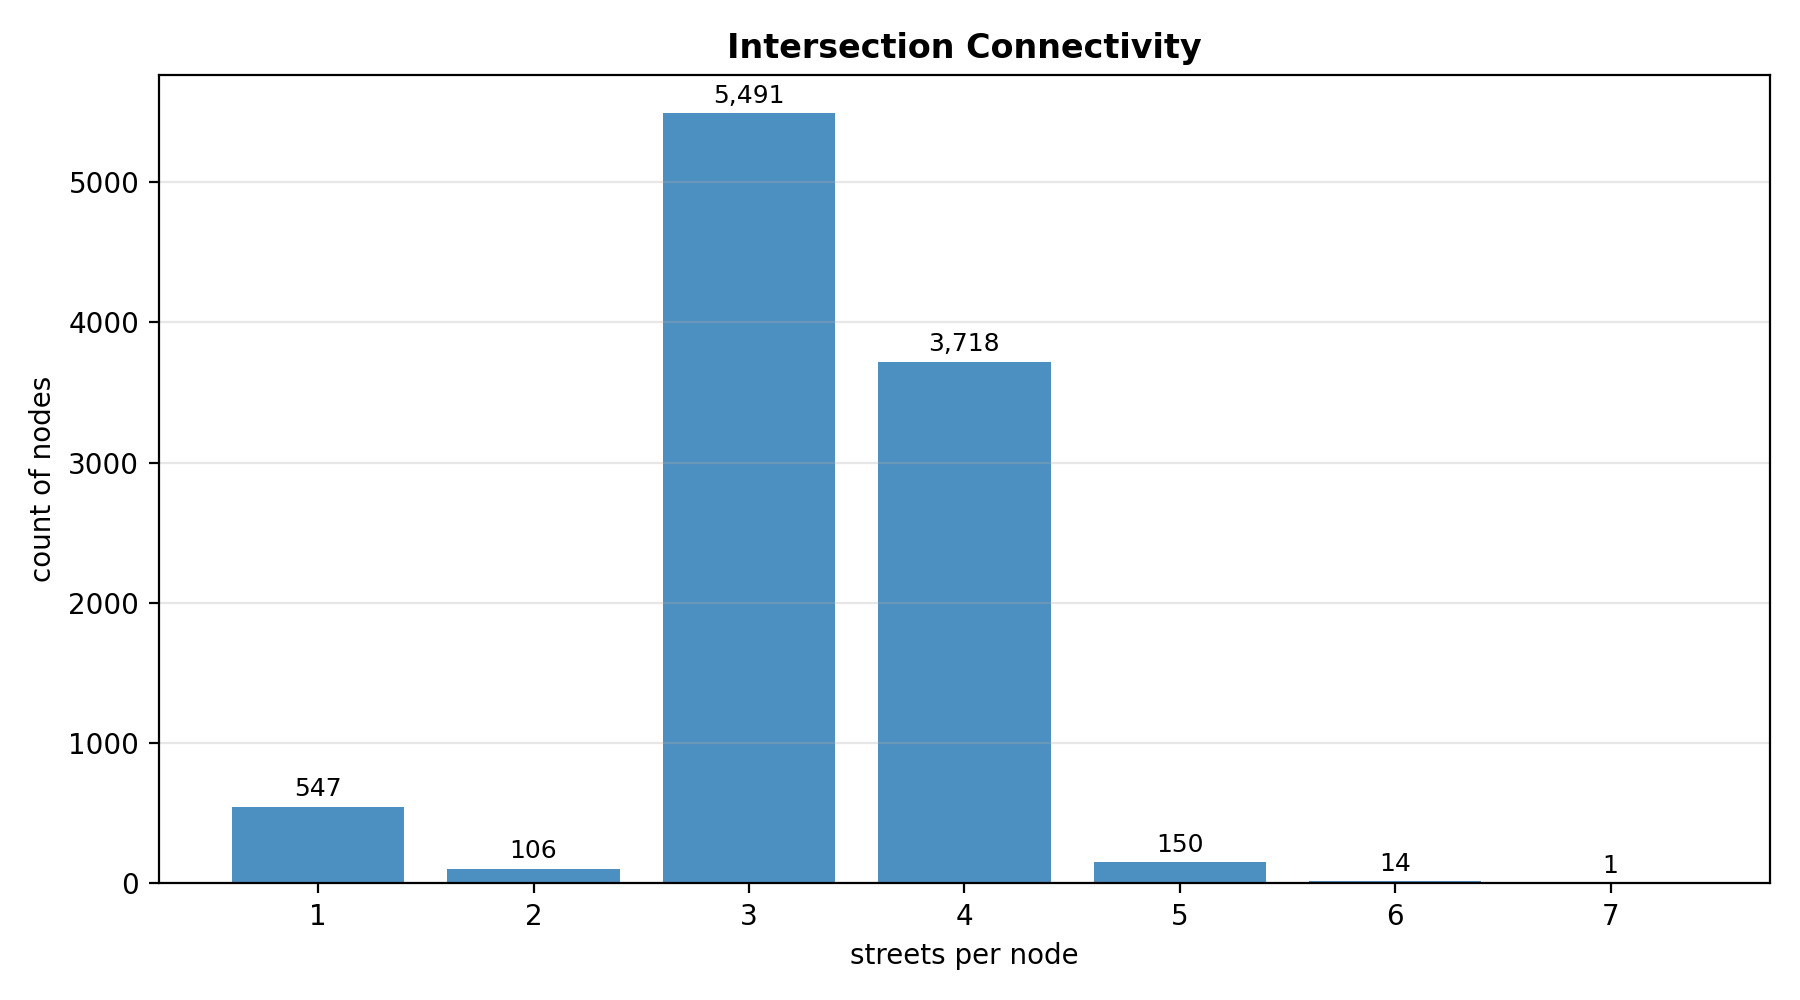
\includegraphics[width=0.8\linewidth,height=\textheight,keepaspectratio]{outputs/02_street_counts.png}

}

\caption{\label{fig-streetcounts}Intersection connectivity across the
network.}

\end{figure}%

As we can see from the plot above, most intersections connect three or
four streets and dead ends are fairly rare, which reflects the L'Enfant
grid. This is a helpful layout for routing, because a courier blocked on
one segment usually has a parallel street right next to it. The
structural analysis asks where that backup runs out.

\begin{figure}[H]

\centering{

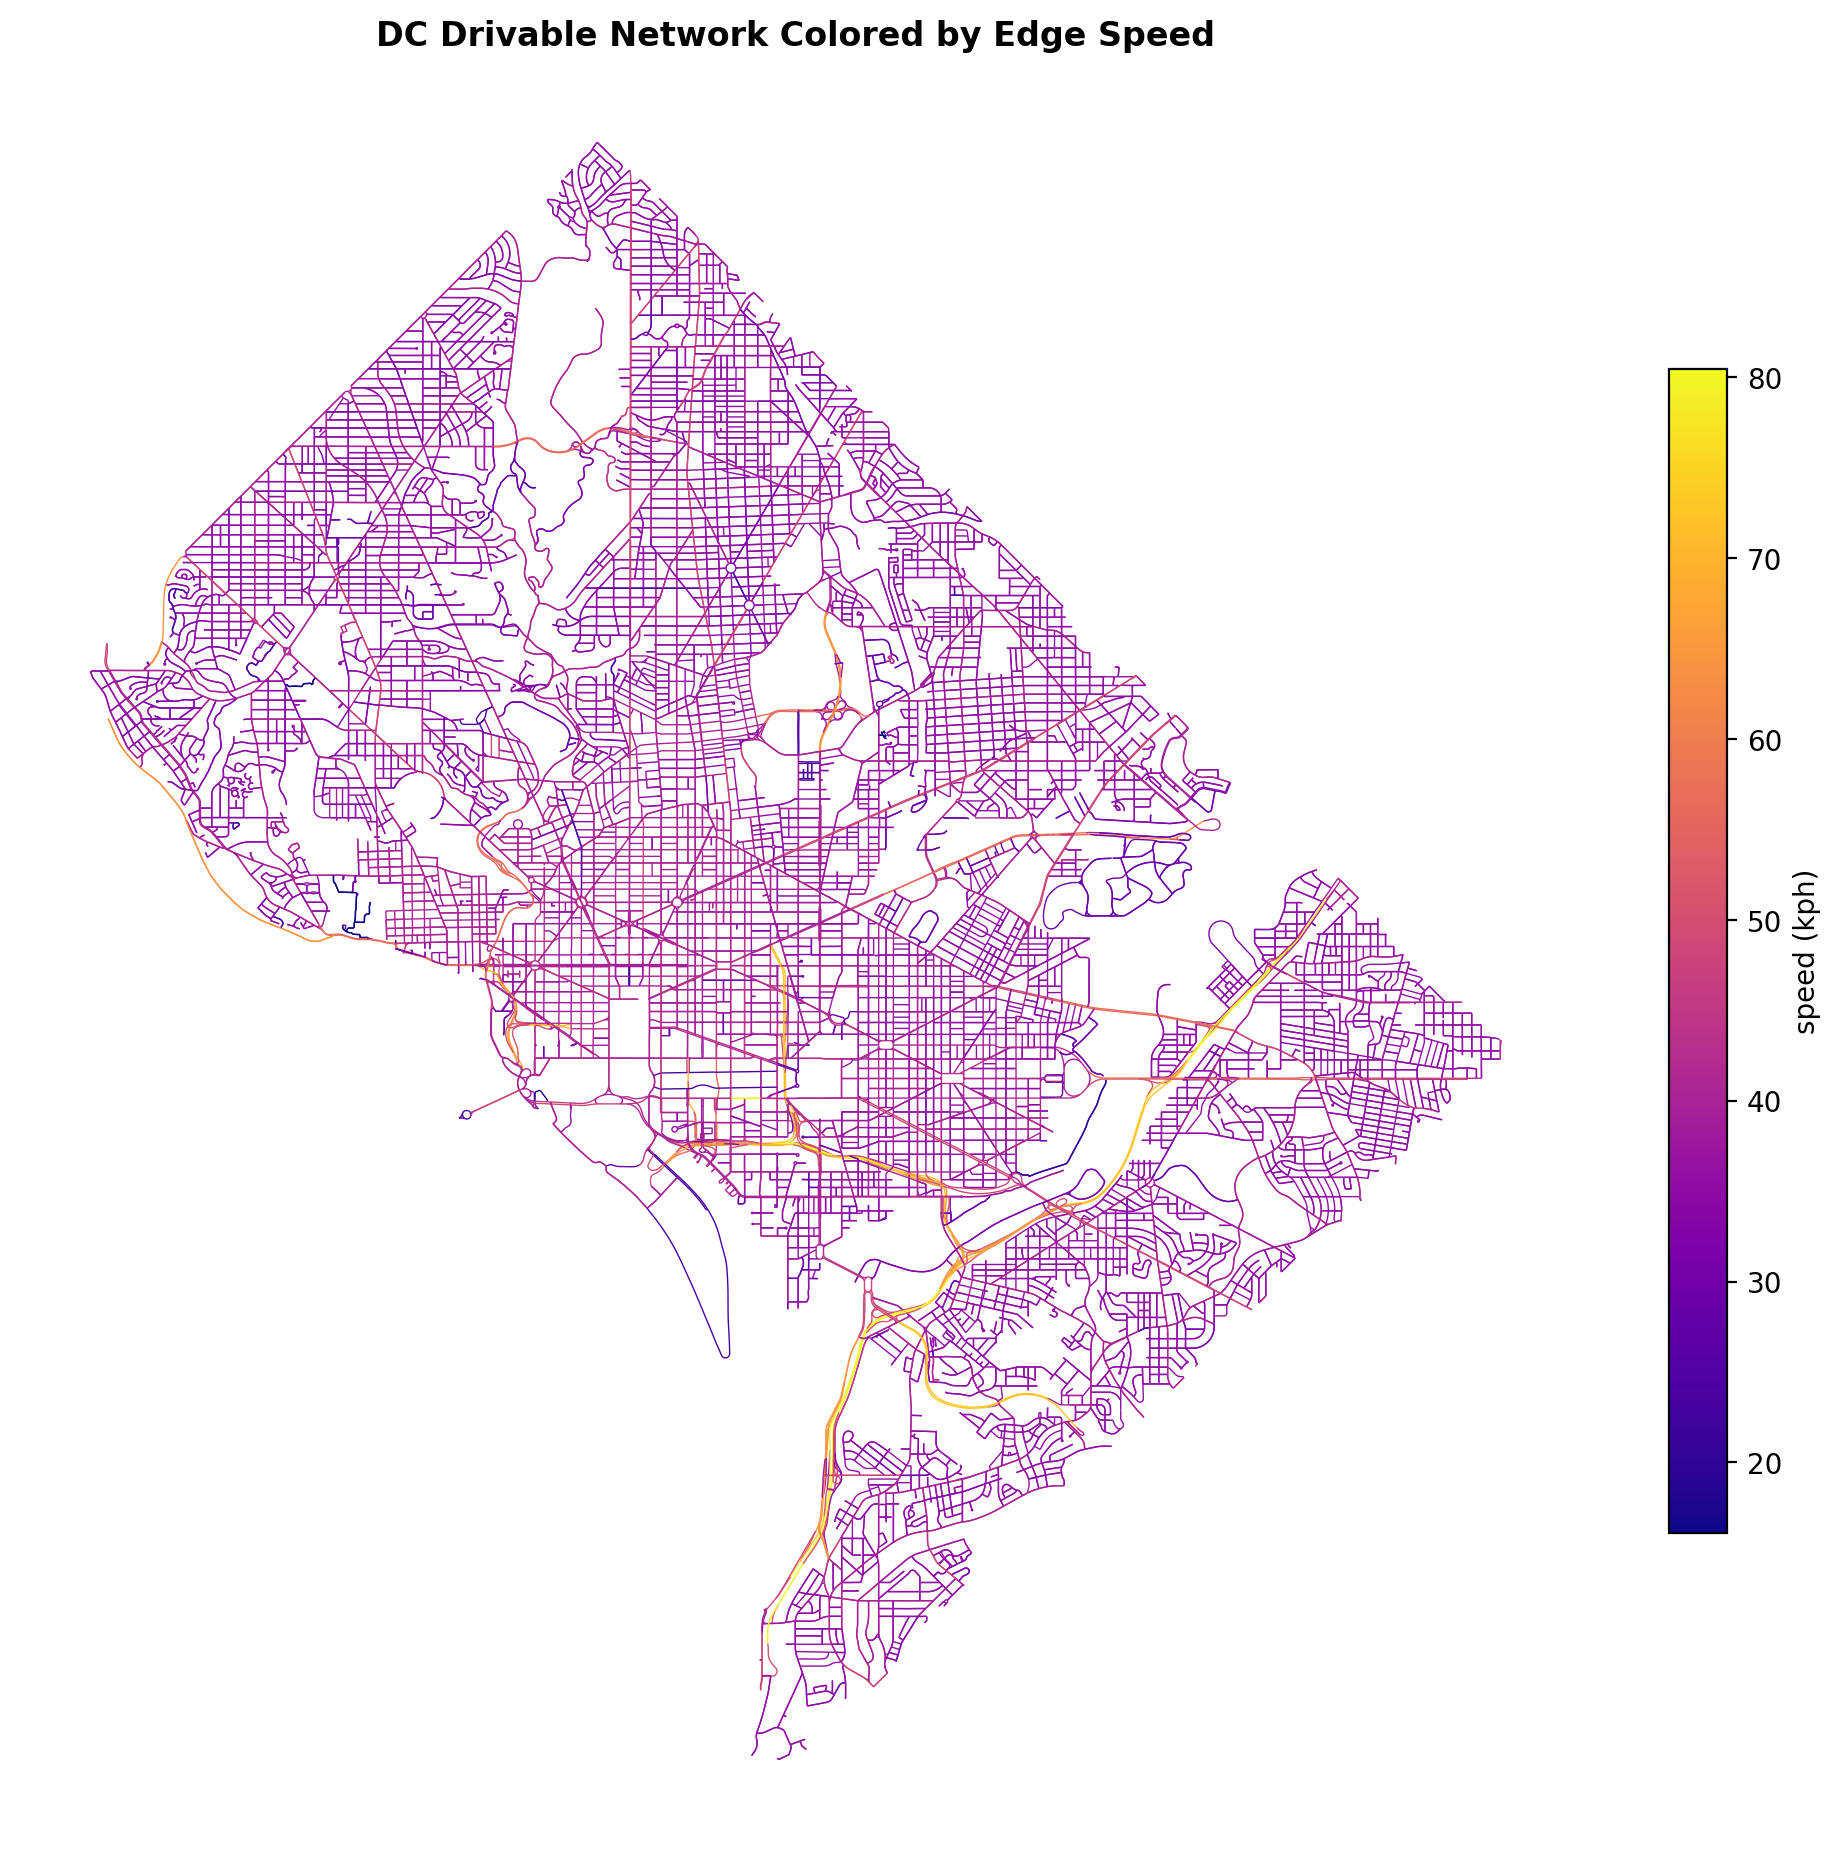
\includegraphics[width=0.85\linewidth,height=\textheight,keepaspectratio]{outputs/01_network_speeds.png}

}

\caption{\label{fig-speeds}The network colored by assigned edge speed.}

\end{figure}%

As we can see from the plot above, the speed structure follows the road
hierarchy we would expect. The interstate segments in the southeast and
the parkway corridors along the rivers carry the highest speeds, the
diagonal avenues sit in the middle, and the large residential fabric
fills in around 35 kph. Deliveries are won or lost on how quickly
couriers can move between these slow local streets and the faster main
roads.

\begin{figure}[H]

\centering{

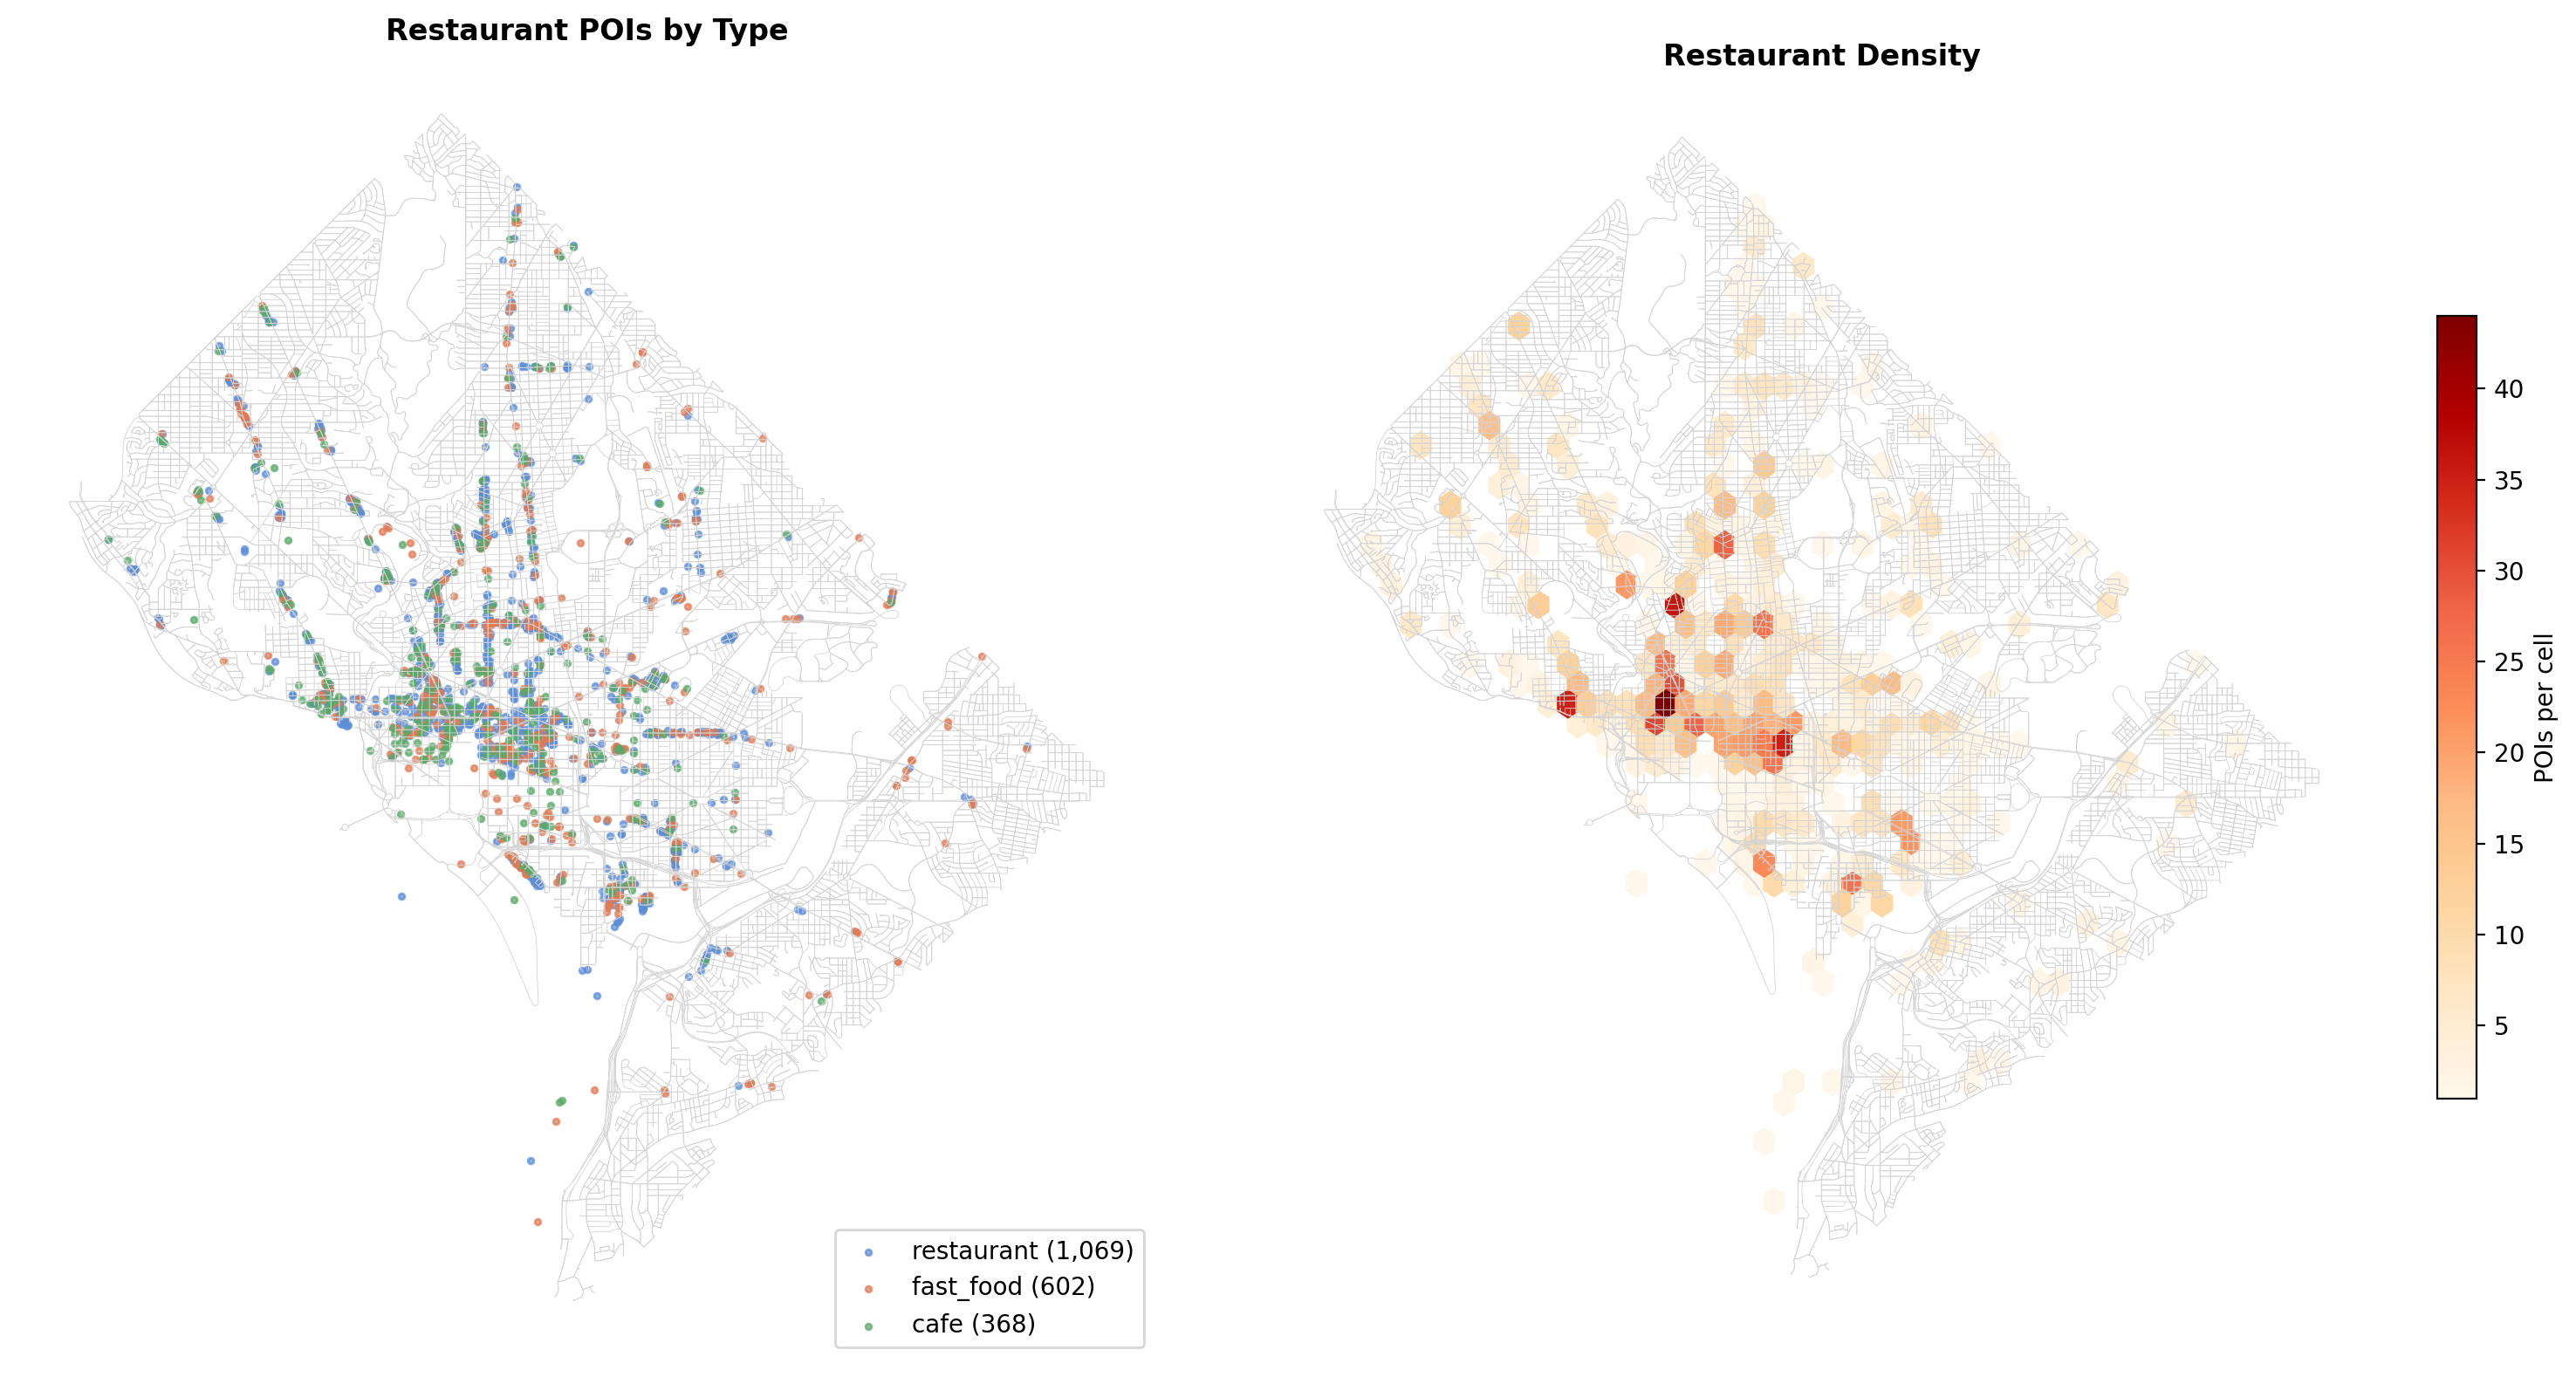
\includegraphics[width=0.95\linewidth,height=\textheight,keepaspectratio]{outputs/03_restaurant_distribution.png}

}

\caption{\label{fig-poidist}Restaurant POIs by type and density.}

\end{figure}%

As we can see from the plot above, the restaurant supply is far from
uniform. Full service restaurants dominate the count, and the density
panel shows sharp concentrations downtown and along the 14th Street, U
Street, H Street, and Georgetown corridors. Large areas east of the
Anacostia River and in the residential northeast have only scattered
supply.

\begin{figure}[H]

\centering{

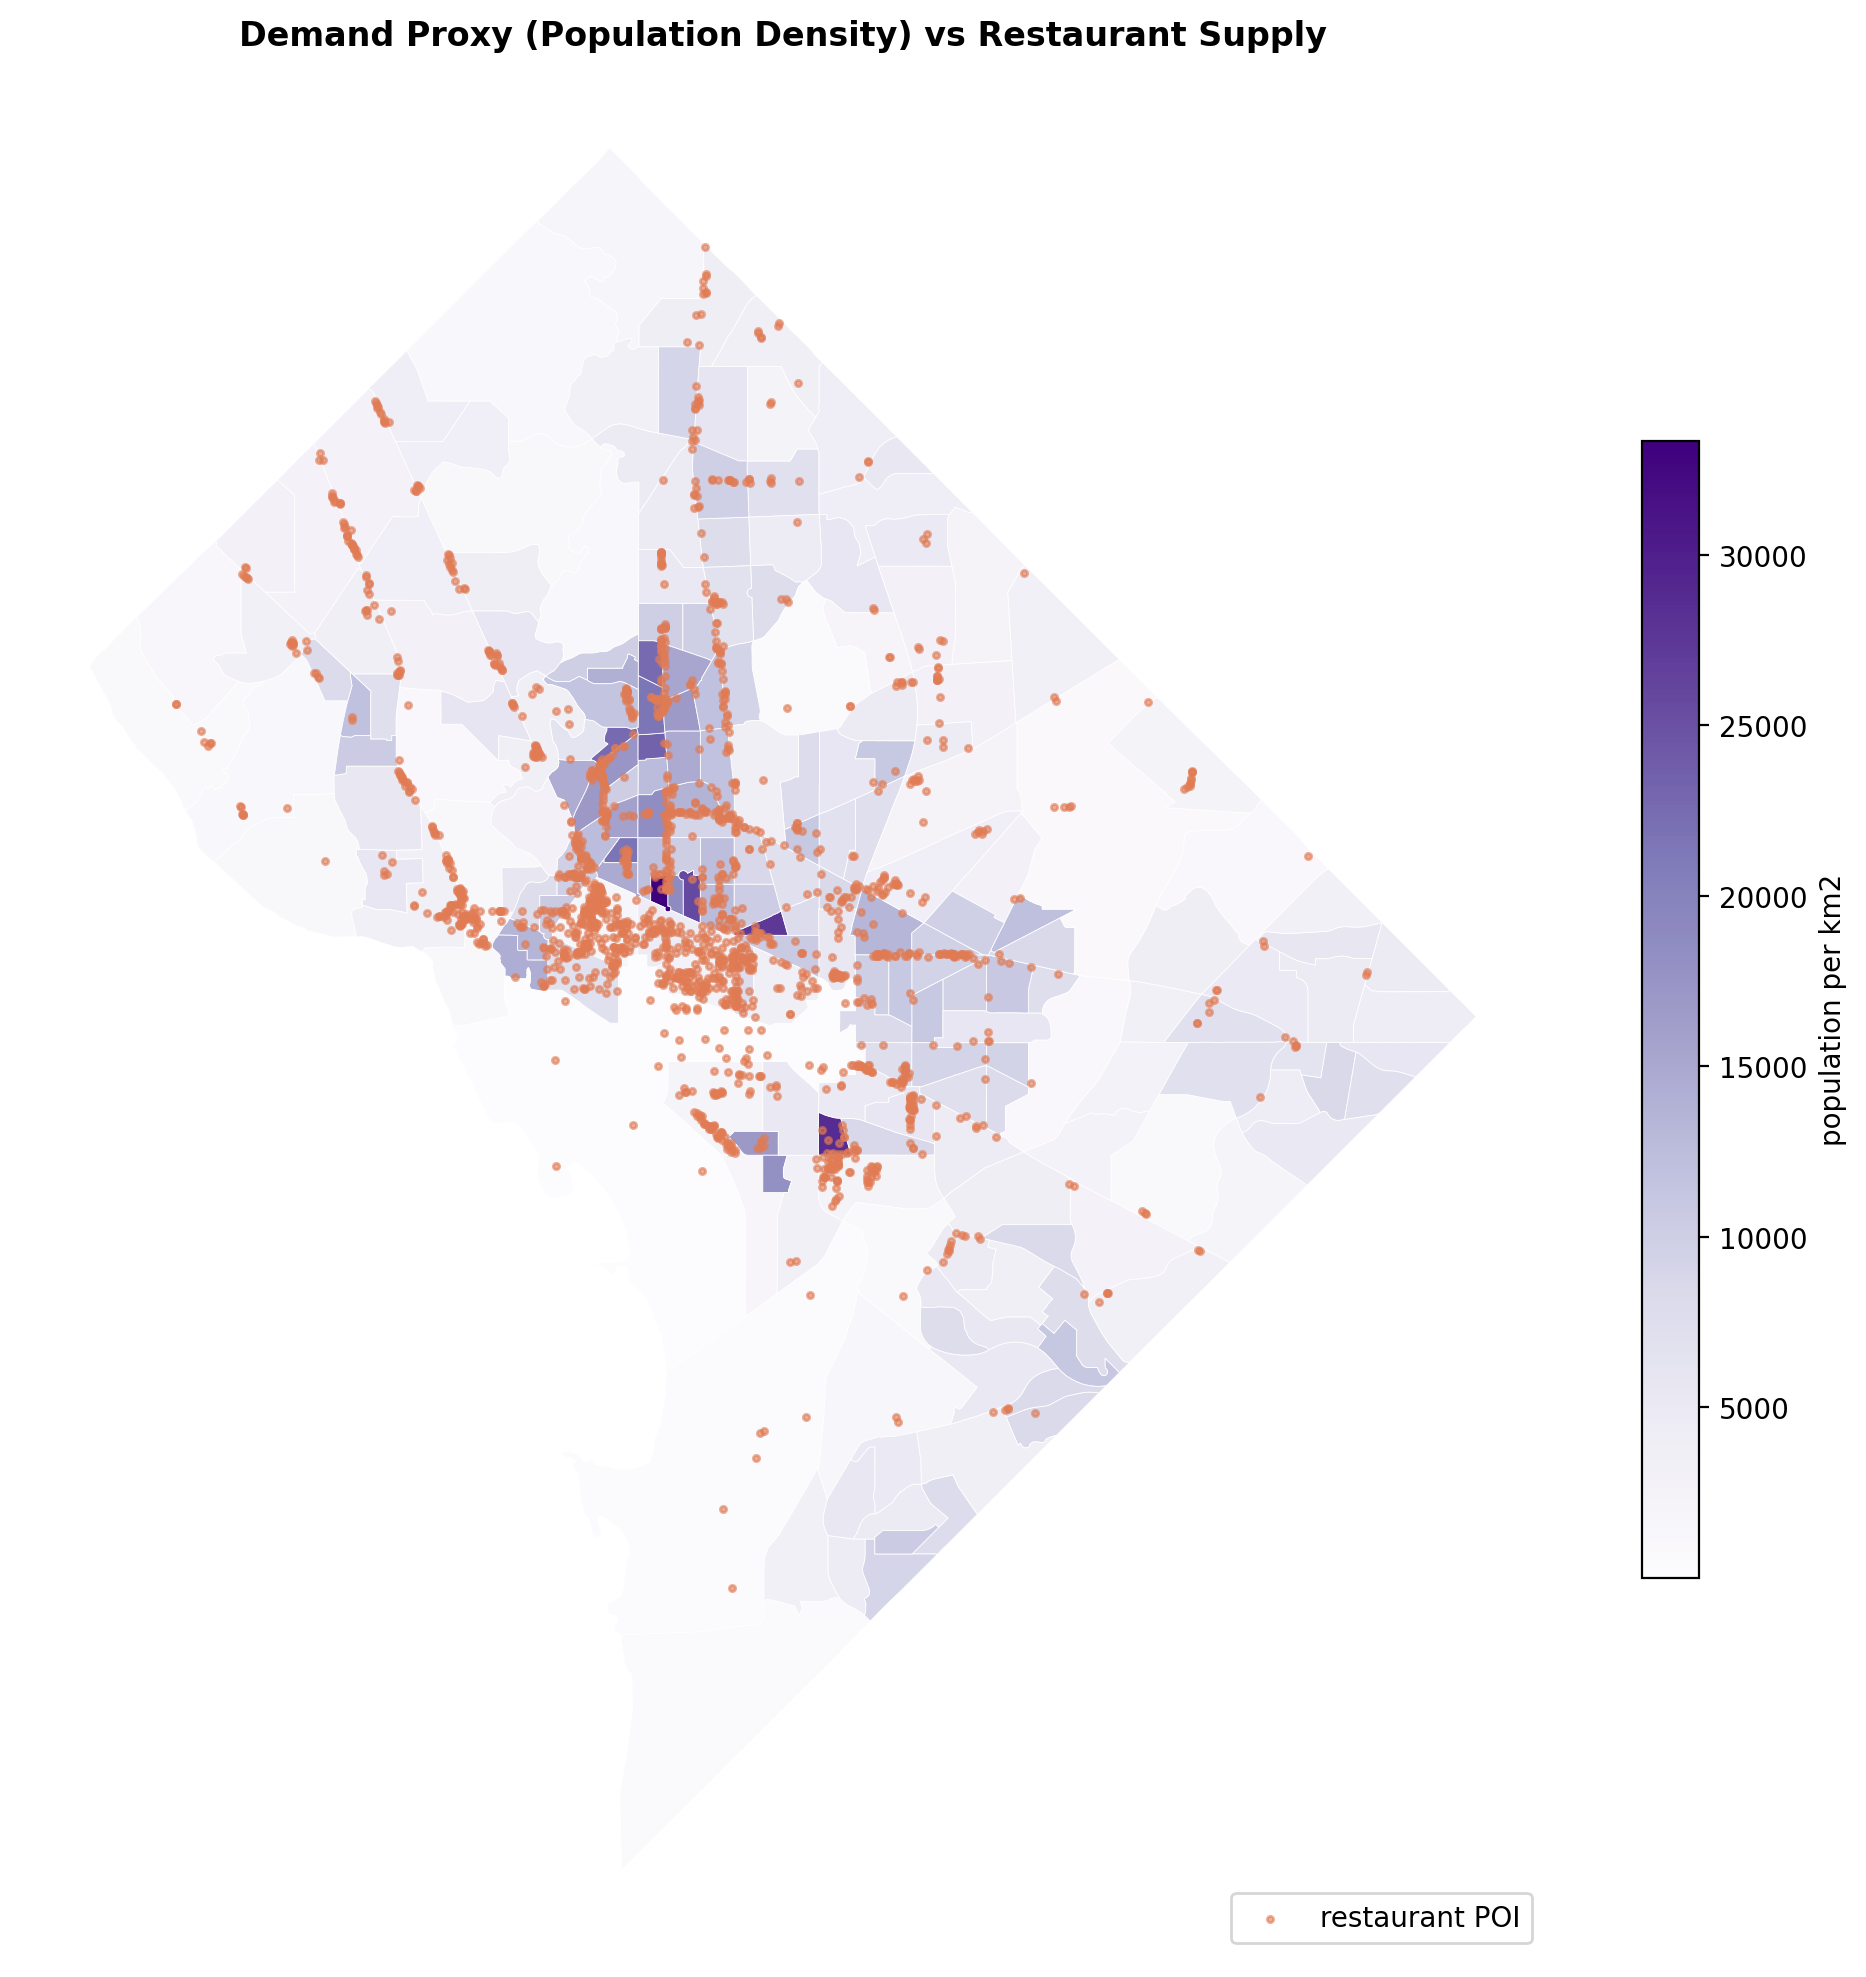
\includegraphics[width=0.85\linewidth,height=\textheight,keepaspectratio]{outputs/05_demand_heatmap.png}

}

\caption{\label{fig-demand}Demand proxy (population density) against
restaurant supply.}

\end{figure}%

As we can see from the plot above, the supply and the demand proxy do
not live in the same places. The ten most restaurant dense tracts hold
37.2 percent of all restaurants but only 4.1 percent of the population,
and the tract level correlation between population and restaurant count
is basically zero at -0.09. Delivery in DC is therefore a transport
problem at its core, because the food is made downtown and in the
northwest corridors while much of the demand lives elsewhere.

\begin{figure}[H]

\centering{

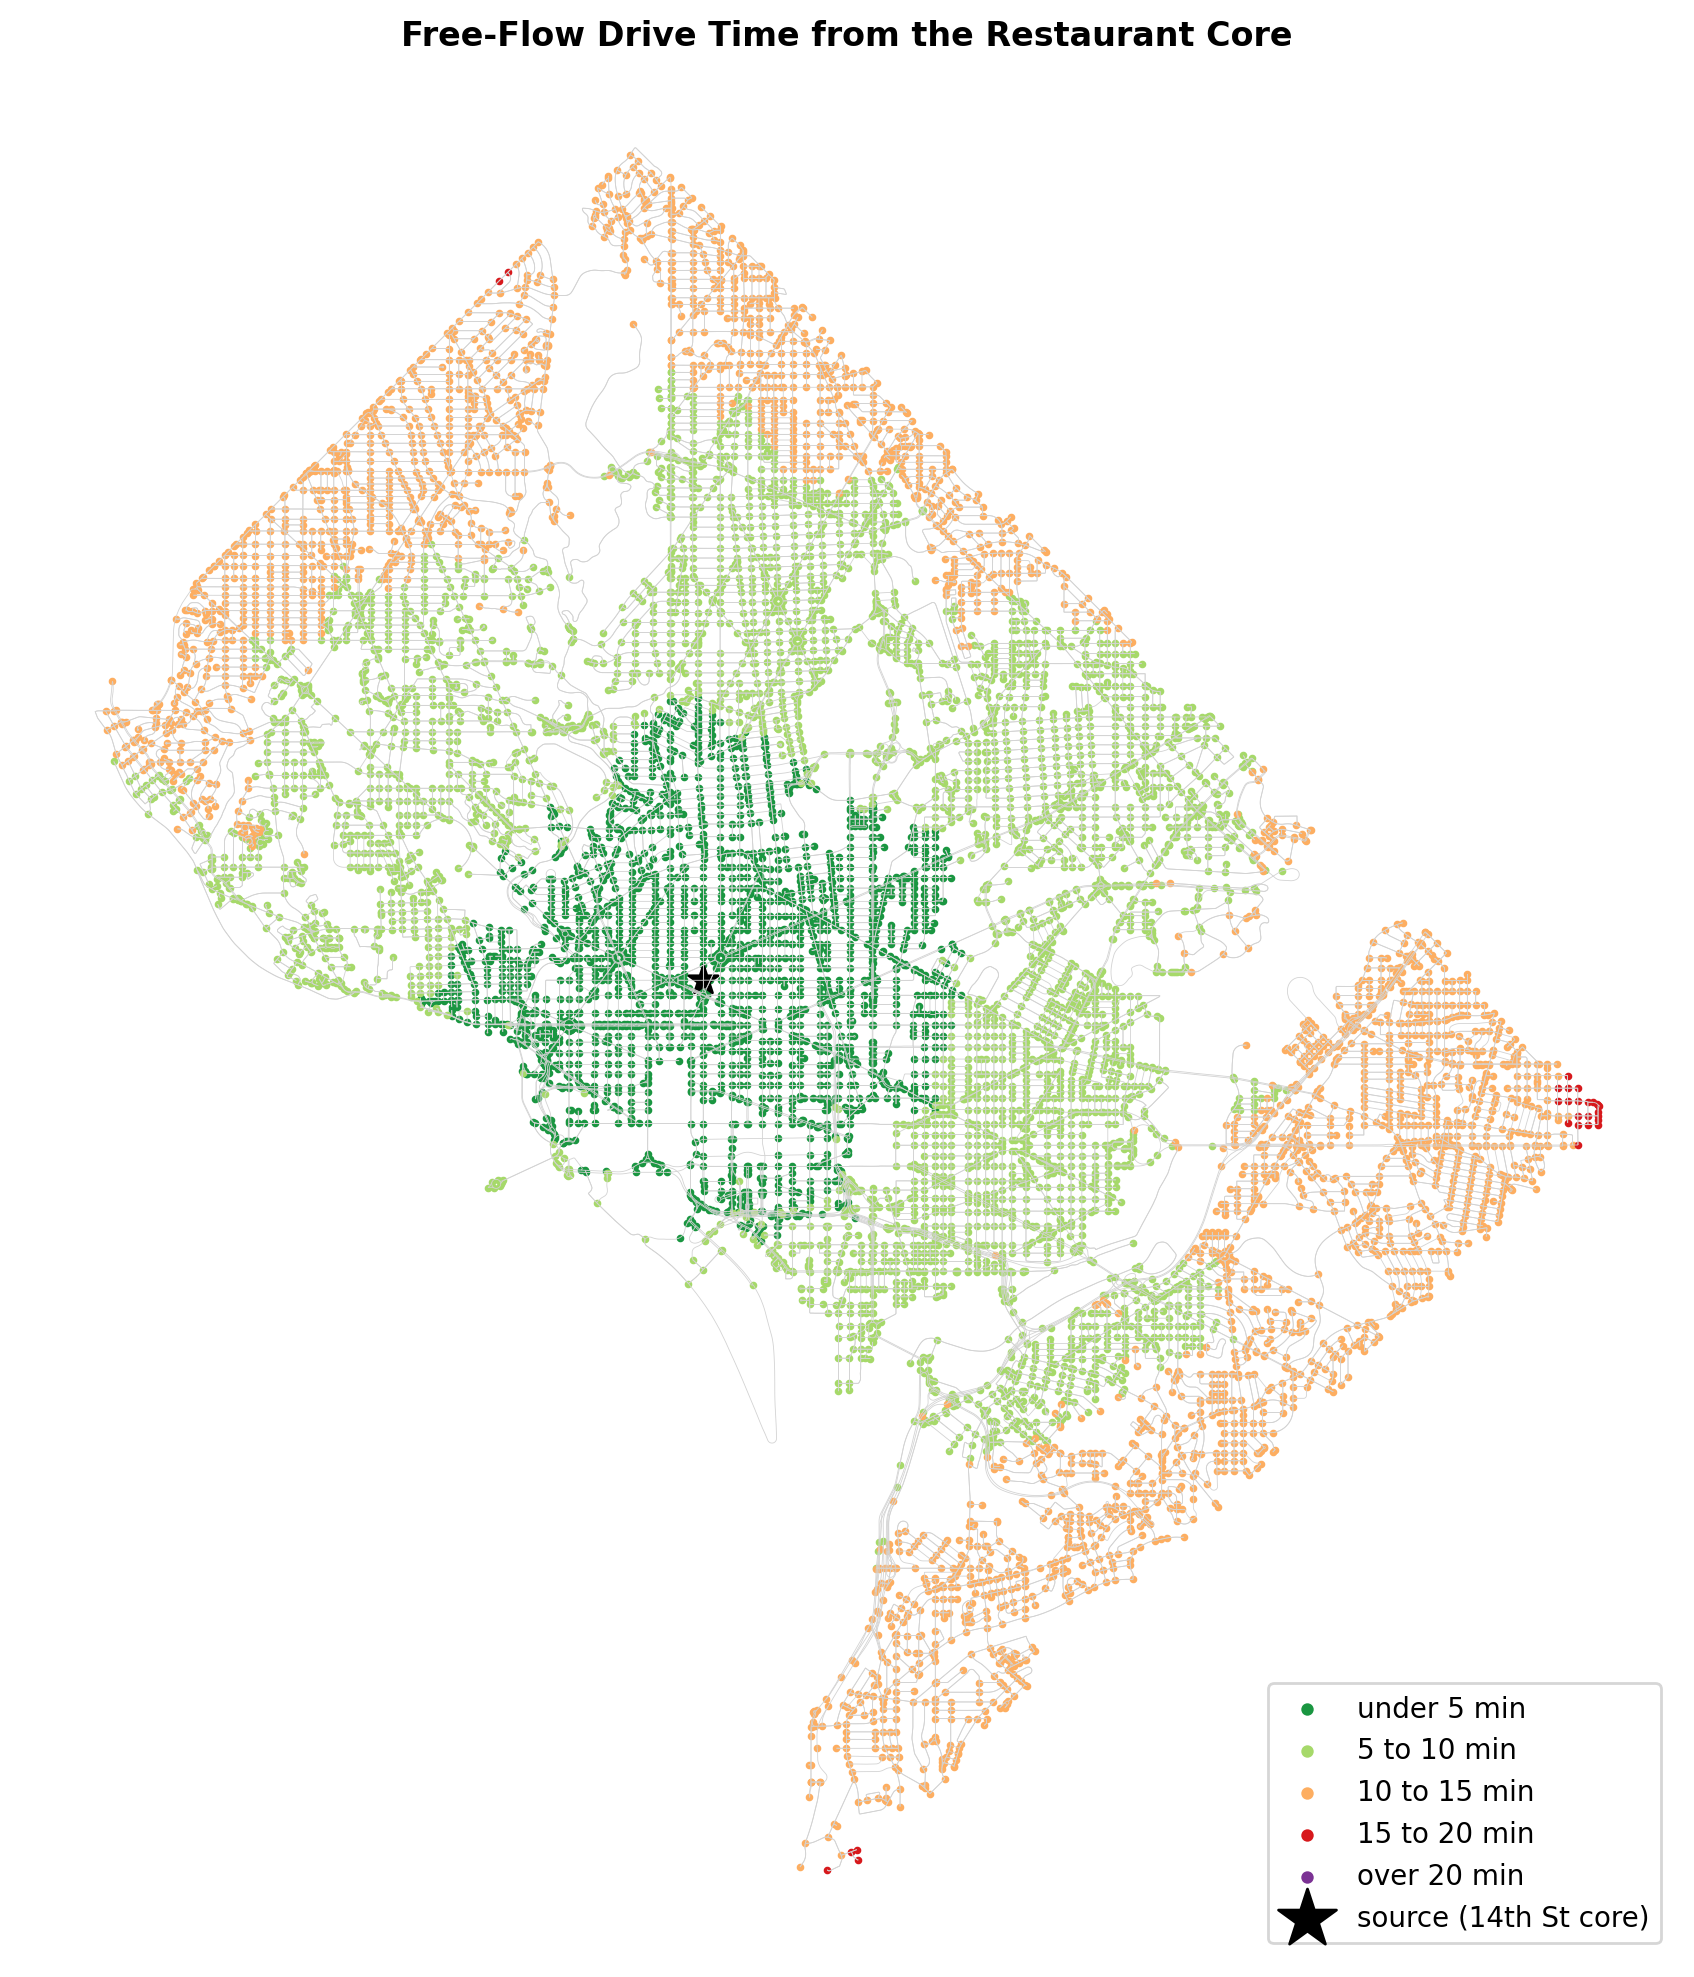
\includegraphics[width=0.85\linewidth,height=\textheight,keepaspectratio]{outputs/07_courier_reach.png}

}

\caption{\label{fig-reach}Free flow drive time from the restaurant
core.}

\end{figure}%

As we can see from the plot above, free flow reach from the 14th Street
core is generous. About 23 percent of intersections are reachable within
five minutes, 68 percent within ten, and nearly the whole District
within fifteen. The catch is that these are free flow times built from
imputed speeds, so real congestion and service overheads will shrink
this picture. The gradient also runs against the demand map, since the
areas beyond the ten minute band are exactly the population dense areas
east of the river.

\section{RQ1: Bottleneck Detection}\label{rq1-bottleneck-detection}

\subsection{Methodology}\label{methodology}

The bottleneck question asks whether simple metrics find the choke
points or whether a more robust method is needed. We compute travel time
weighted edge betweenness centrality, approximated over 150 sampled
sources, which estimates the share of shortest paths that cross each
edge. Joshi et al. (2022) use the same idea when they precompute
shortest path structure for assignment in dynamic road networks. We then
compare the betweenness ranking against observed AADT and against edge
speed, the two simple options someone would try first, using Spearman
rank correlation and the overlap between the top one percent sets.

\subsection{Results}\label{results}

\begin{figure}[H]

\centering{

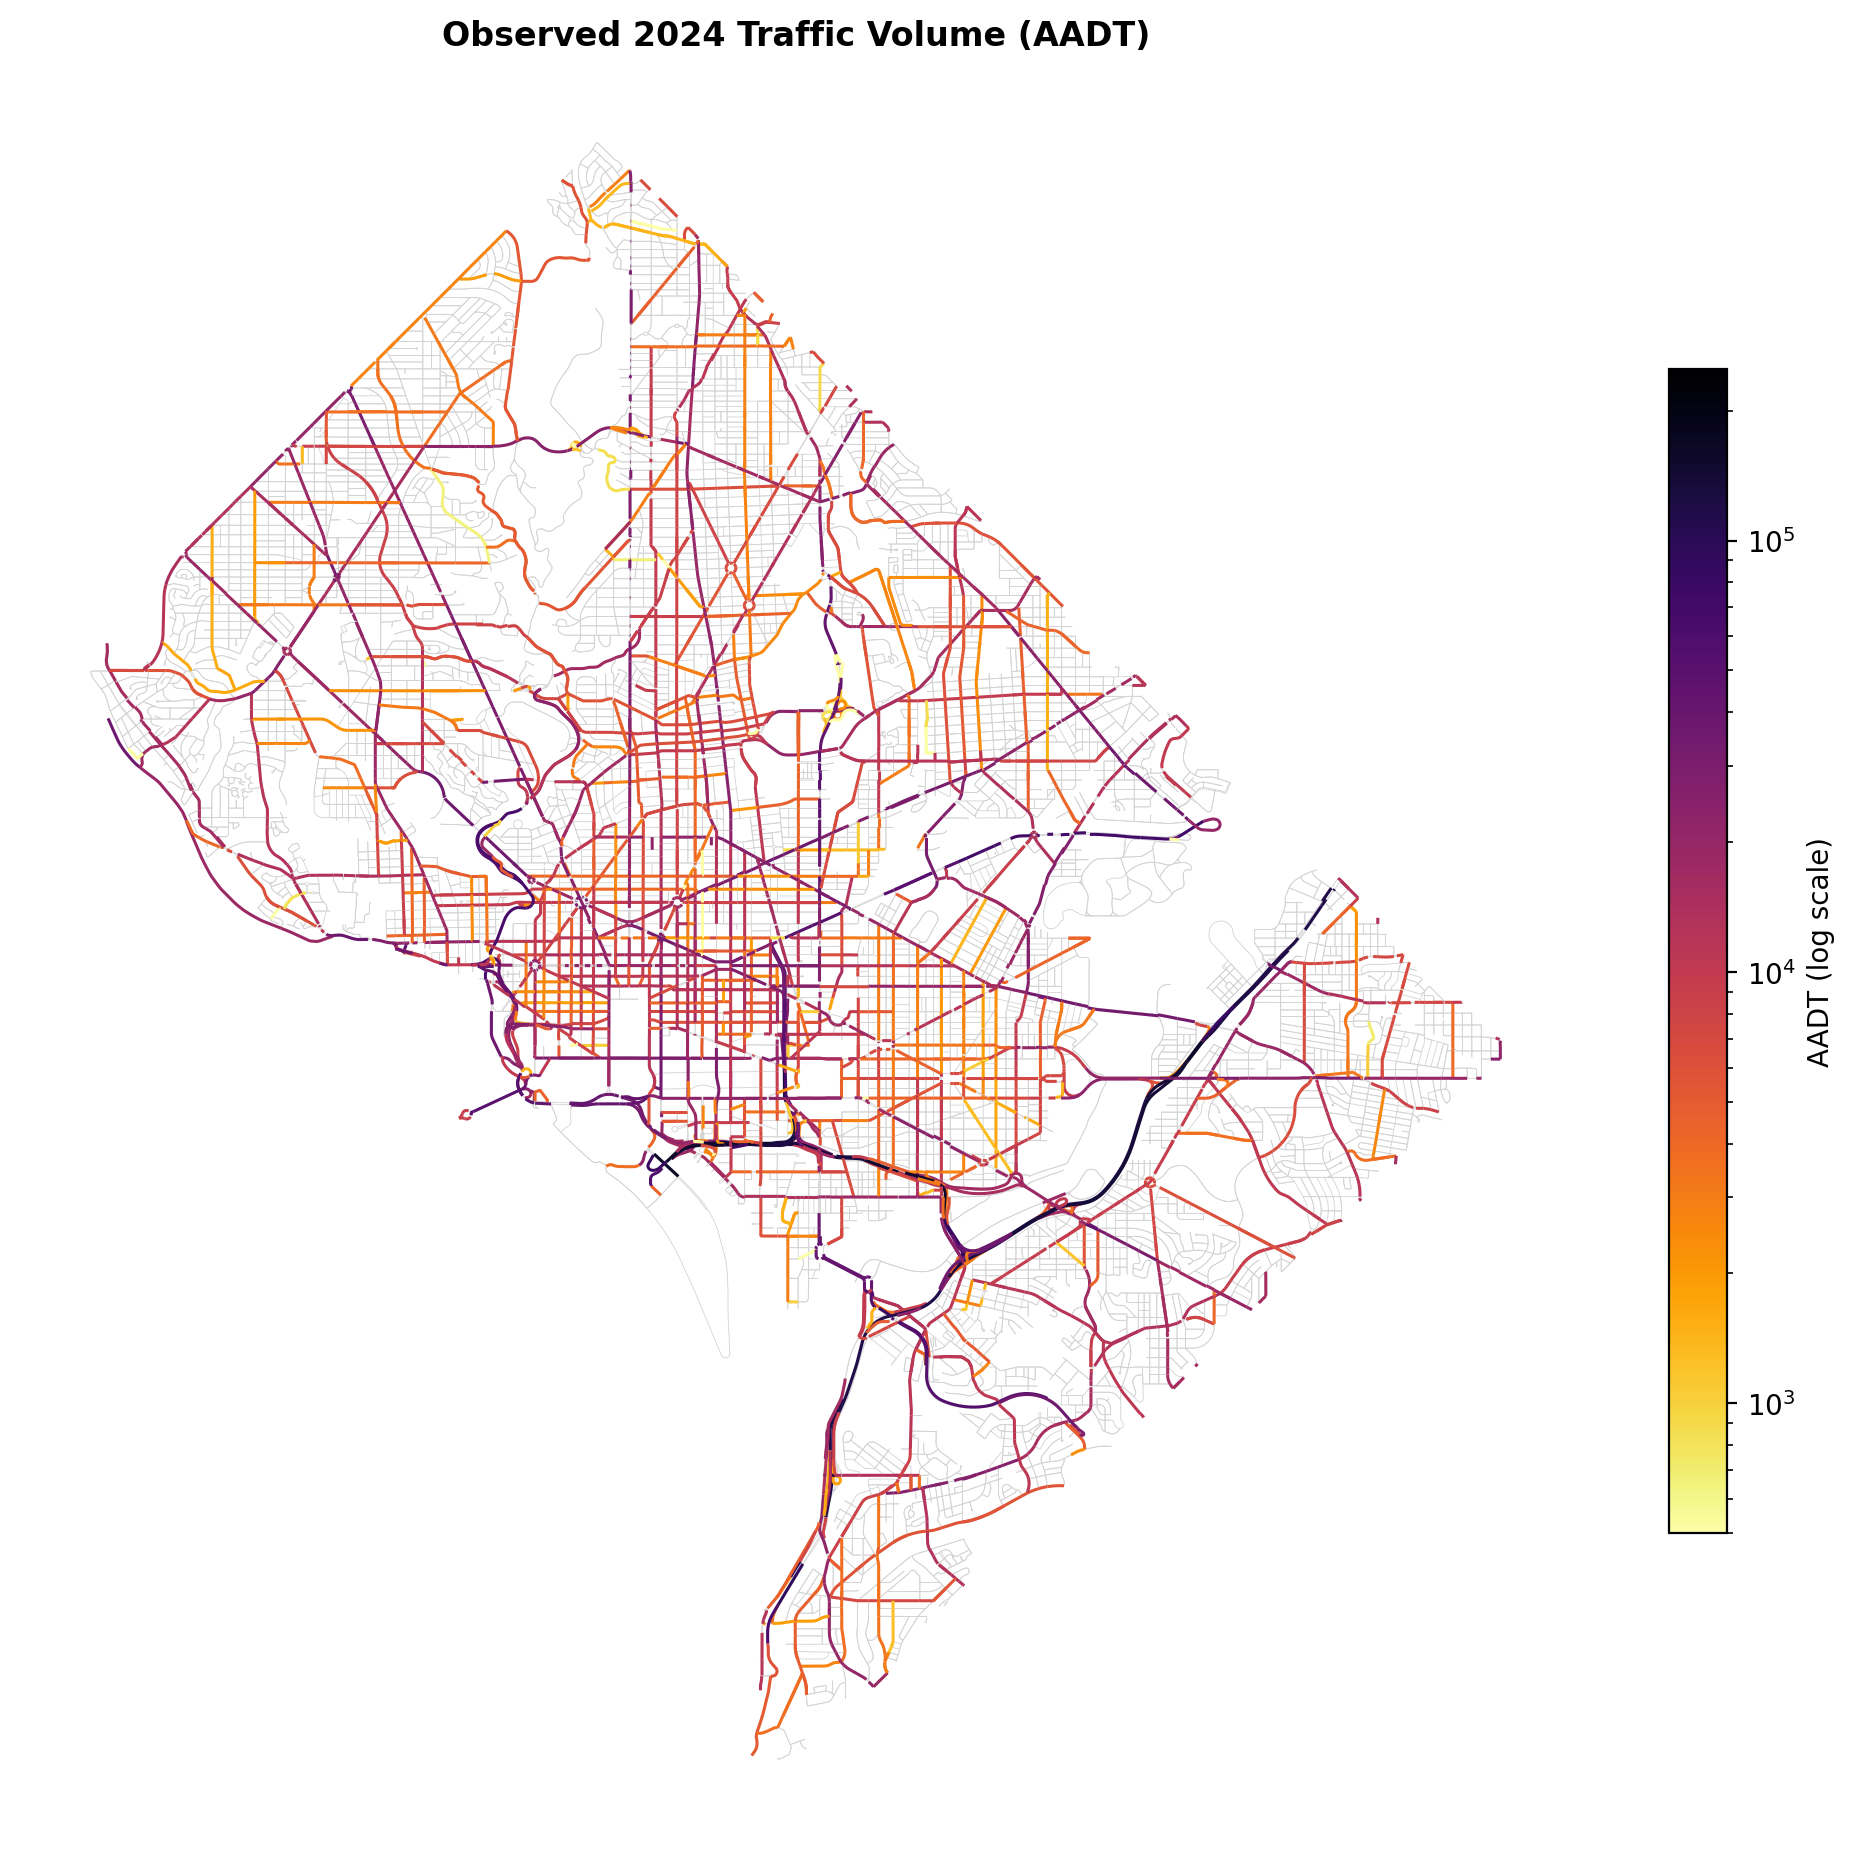
\includegraphics[width=0.85\linewidth,height=\textheight,keepaspectratio]{outputs/06_traffic_aadt.png}

}

\caption{\label{fig-aadt}Observed 2024 traffic volume (AADT) on the DC
network.}

\end{figure}%

As we can see from the plot above, observed traffic volume concentrates
on the freeway spine, the river bridges, and a small set of surface
arterials. Volume alone, however, is not structure. The Spearman rank
correlation between betweenness and observed AADT is 0.42 on monitored
edges, and 0.58 between betweenness and free flow speed, but the top one
percent of edges by AADT and by betweenness overlap by just 8 percent.

\begin{figure}[H]

\centering{

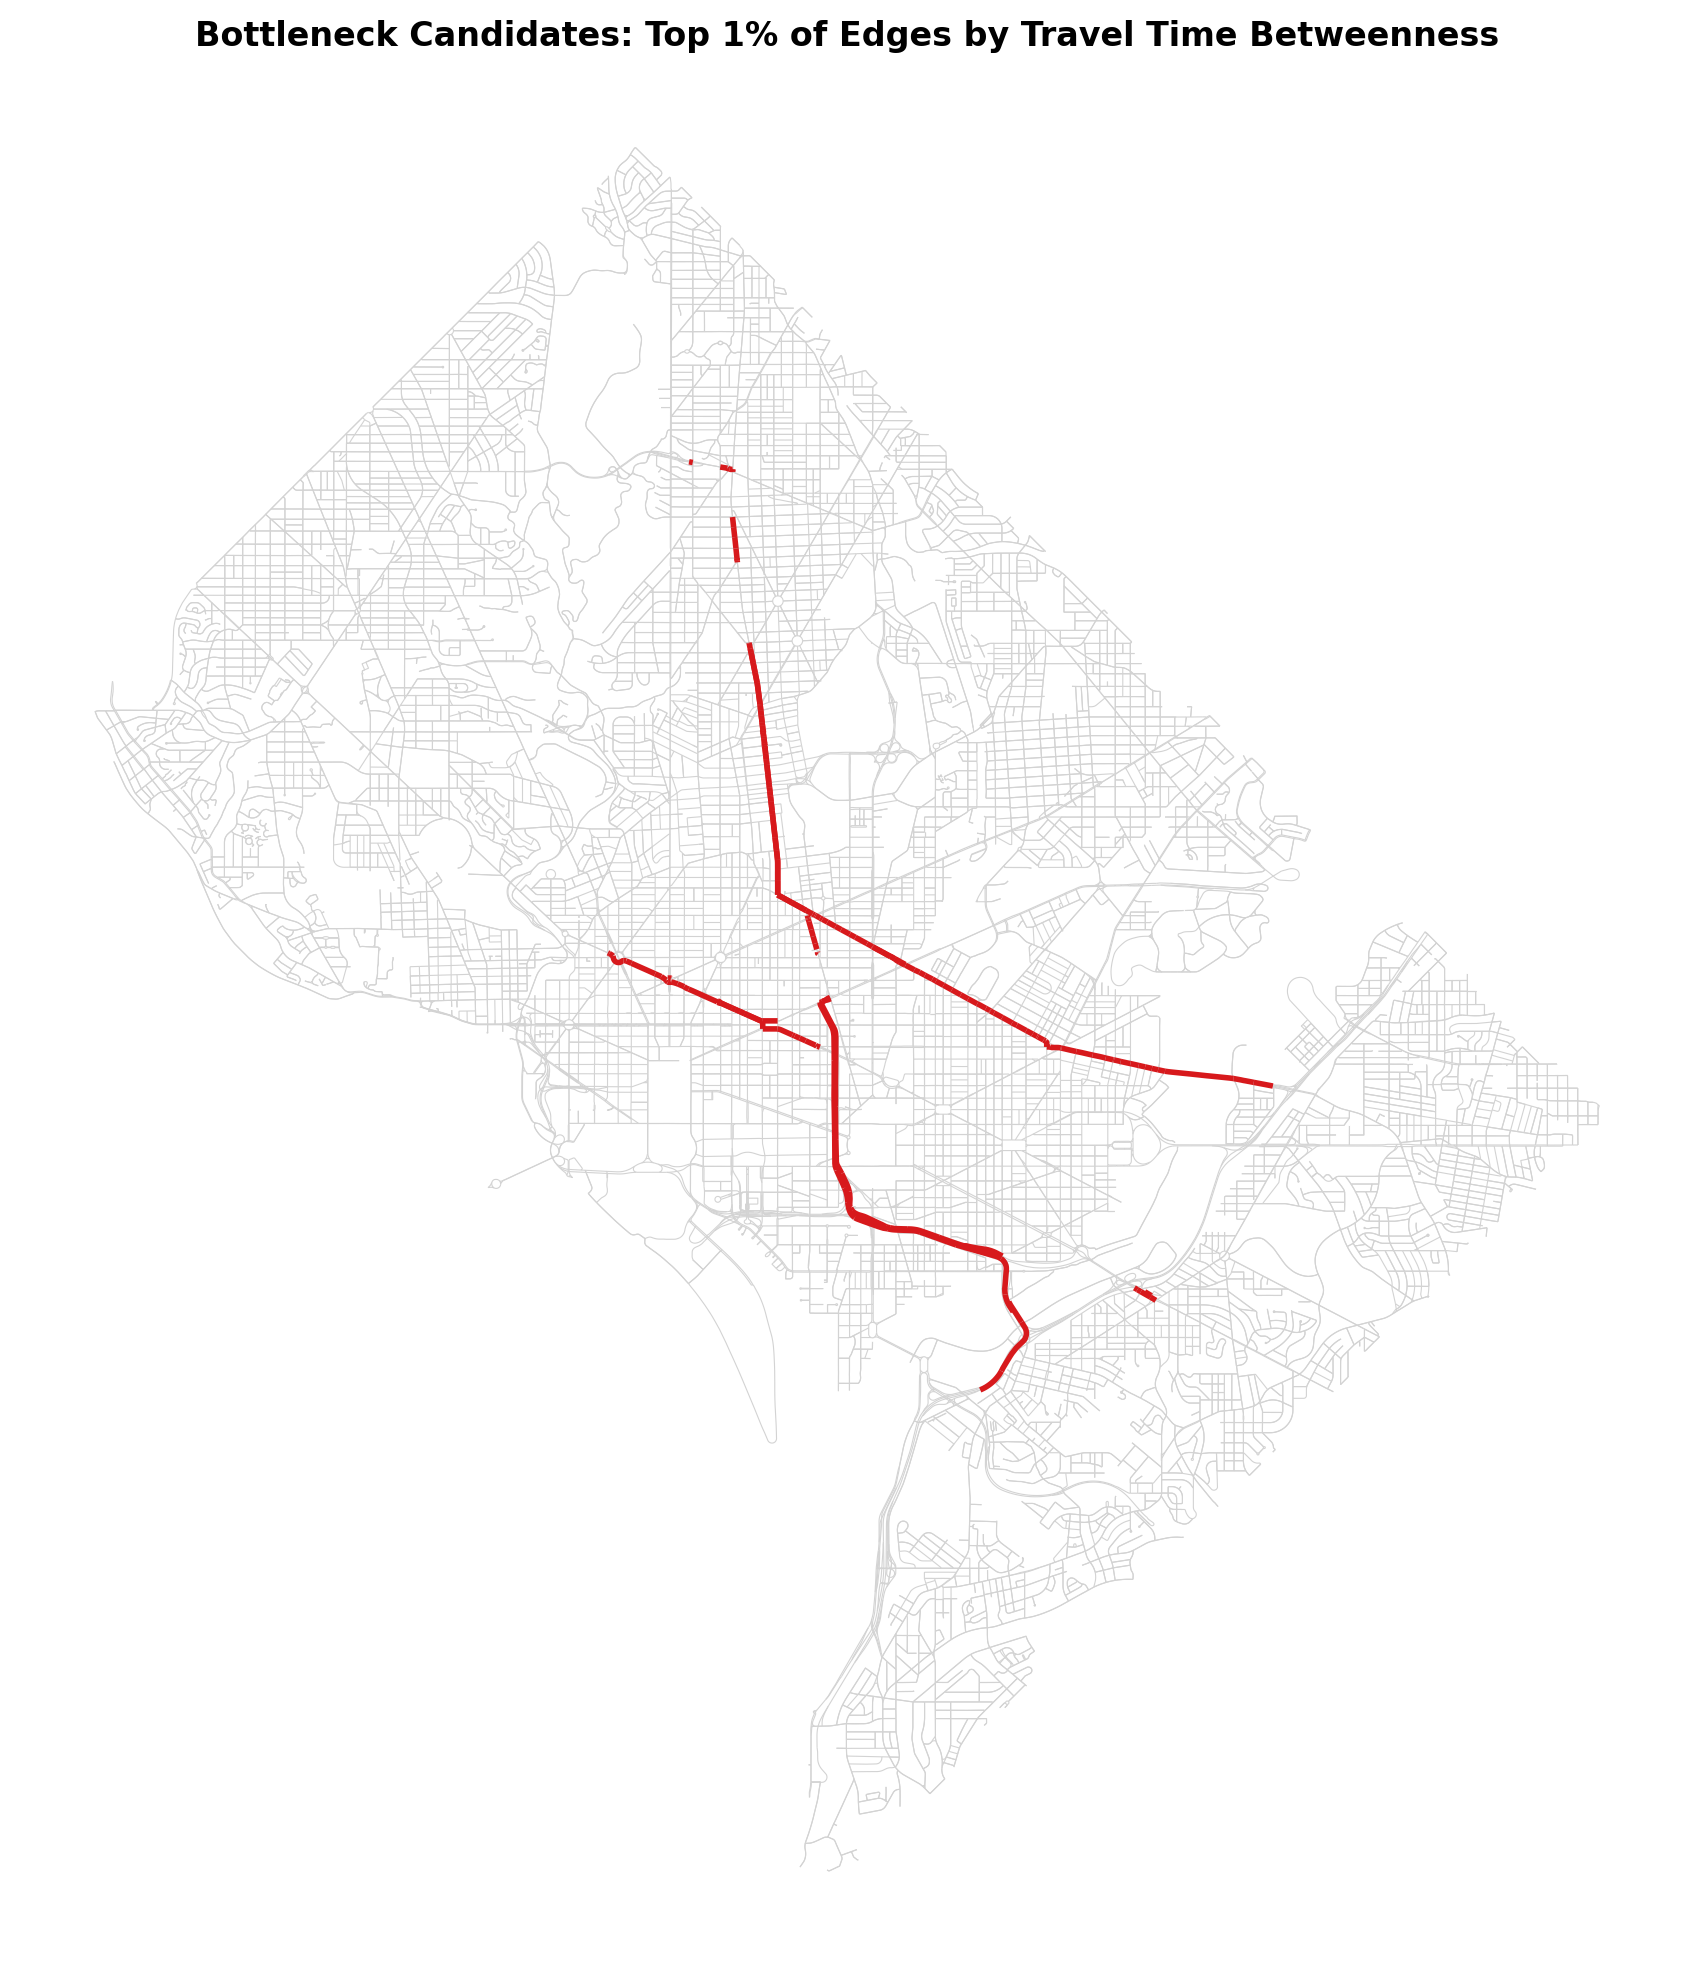
\includegraphics[width=0.85\linewidth,height=\textheight,keepaspectratio]{outputs/08_bottleneck_edges.png}

}

\caption{\label{fig-bottlenecks}Top one percent of edges by travel time
weighted betweenness.}

\end{figure}%

As we can see from the plot above, the betweenness ranking concentrates
on a short list of crossings led by the 3rd Street Tunnel and the
Southeast Freeway, with Florida Avenue the leading surface street. These
are the true chokepoints in the sense that shortest paths have no good
way around them. The answer to RQ1 is that simple metrics are useful
backup evidence but would miss most of the chokepoints, so the path
based measure is needed.

\section{RQ2: Demand Ceiling}\label{rq2-demand-ceiling}

\subsection{Methodology}\label{methodology-1}

The demand ceiling question asks whether there is an order volume the
network simply cannot move fast enough to meet. We answer it with
throughput arithmetic on the simulation setup. The mean busy cycle per
delivery, measured in uncongested reference runs, converts into how many
orders one courier can complete per hour. Comparing that capacity
against the arrival profile of the synthetic day shows the rate at which
a given fleet gets overwhelmed.

\subsection{Results}\label{results-1}

An uncongested courier completes about 2.9 orders per hour given the
20.5 minute busy cycle, so holding the 2,279 order 19:00 peak without a
growing queue would take roughly 780 couriers. A 500 courier fleet, the
size that meets the daily service standard in the operational analysis,
caps out near 1,461 orders per hour. It survives the rush only because
the peak is short enough for the backlog to drain afterward. Daily
volume is not the problem, since that same fleet could move about 35,000
orders in a flat day. The answer to RQ2 is that the ceiling is a limit
on orders per hour rather than on total daily orders, near 1,500 per
hour at fleet 500, and it binds at dinner.

\section{RQ3: Renovation Targets}\label{rq3-renovation-targets}

\subsection{Methodology}\label{methodology-2}

The renovation question asks which roads give the most improvement if
upgraded. We run a simple counterfactual on a common origin destination
sample of 320 restaurant to demand pairs. The highest betweenness
surface edges with speeds below 40 kph, seven edges under the current
threshold, are raised to a 48 kph arterial standard, travel times are
recomputed, and the change in mean OD travel time is measured. Three
upgrades of the same number of random slow edges serve as the control.

\subsection{Results}\label{results-2}

\begin{figure}[H]

\centering{

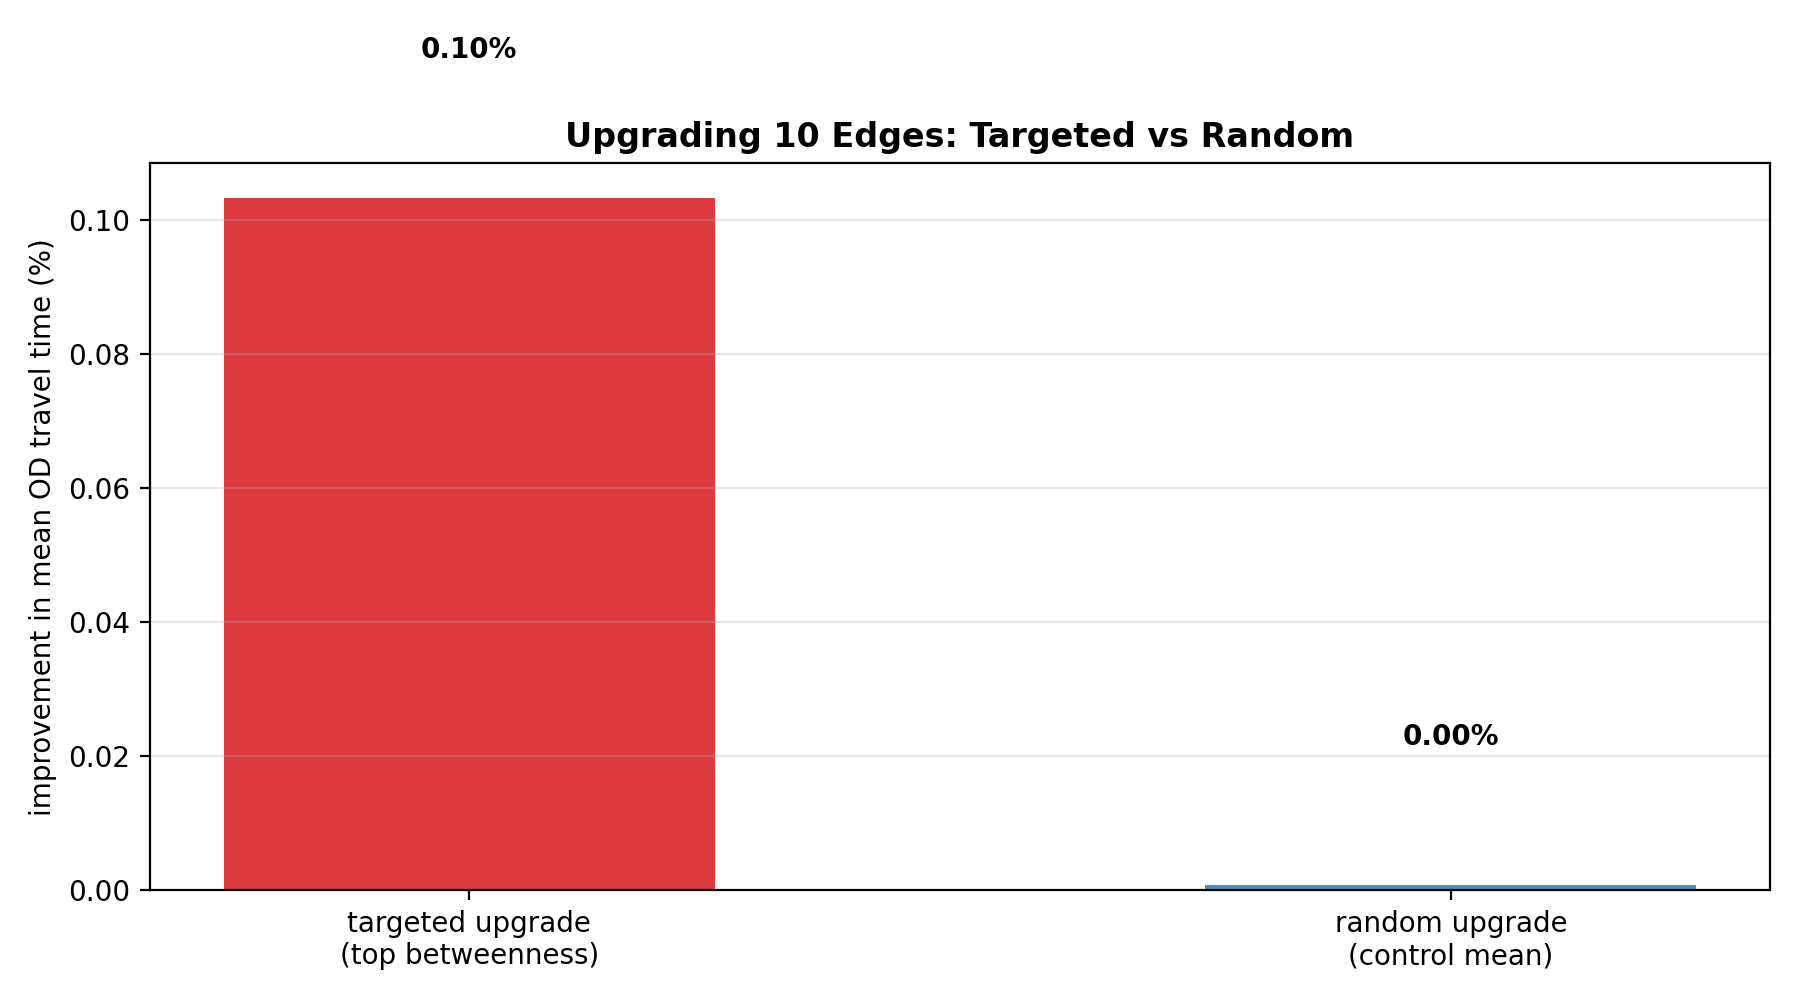
\includegraphics[width=0.7\linewidth,height=\textheight,keepaspectratio]{outputs/09_renovation_experiment.png}

}

\caption{\label{fig-renovation}Improvement in mean OD travel time from
the targeted upgrade.}

\end{figure}%

As we can see from the plot above, the targeted upgrade lands on Florida
Avenue NW and New Jersey Avenue NW and improves mean travel time by
about 0.09 percent, while an equal sized random upgrade does basically
nothing. Targeting by betweenness works, but no handful of edge fixes
meaningfully changes citywide delivery times, because the slow part of a
delivery is the residential last leg rather than any single arterial
segment. Renovation budgets should follow the betweenness ranking with
expectations set at corridor scale.

\section{RQ4: Restaurant Clustering}\label{rq4-restaurant-clustering}

\subsection{Methodology}\label{methodology-3}

The clustering question has two halves. The first asks whether DC
restaurants cluster more than chance would produce, which we measure
with nearest neighbor distances against a uniform random baseline inside
the DC boundary, summarized with the Clark-Evans ratio. The second asks
whether being inside a cluster helps or hurts access to demand. We
compare restaurants with at least ten neighbors within 250 m against
effectively isolated restaurants, measuring mean network travel time
from each group to the same population weighted demand sample.

\subsection{Results}\label{results-3}

\begin{figure}[H]

\centering{

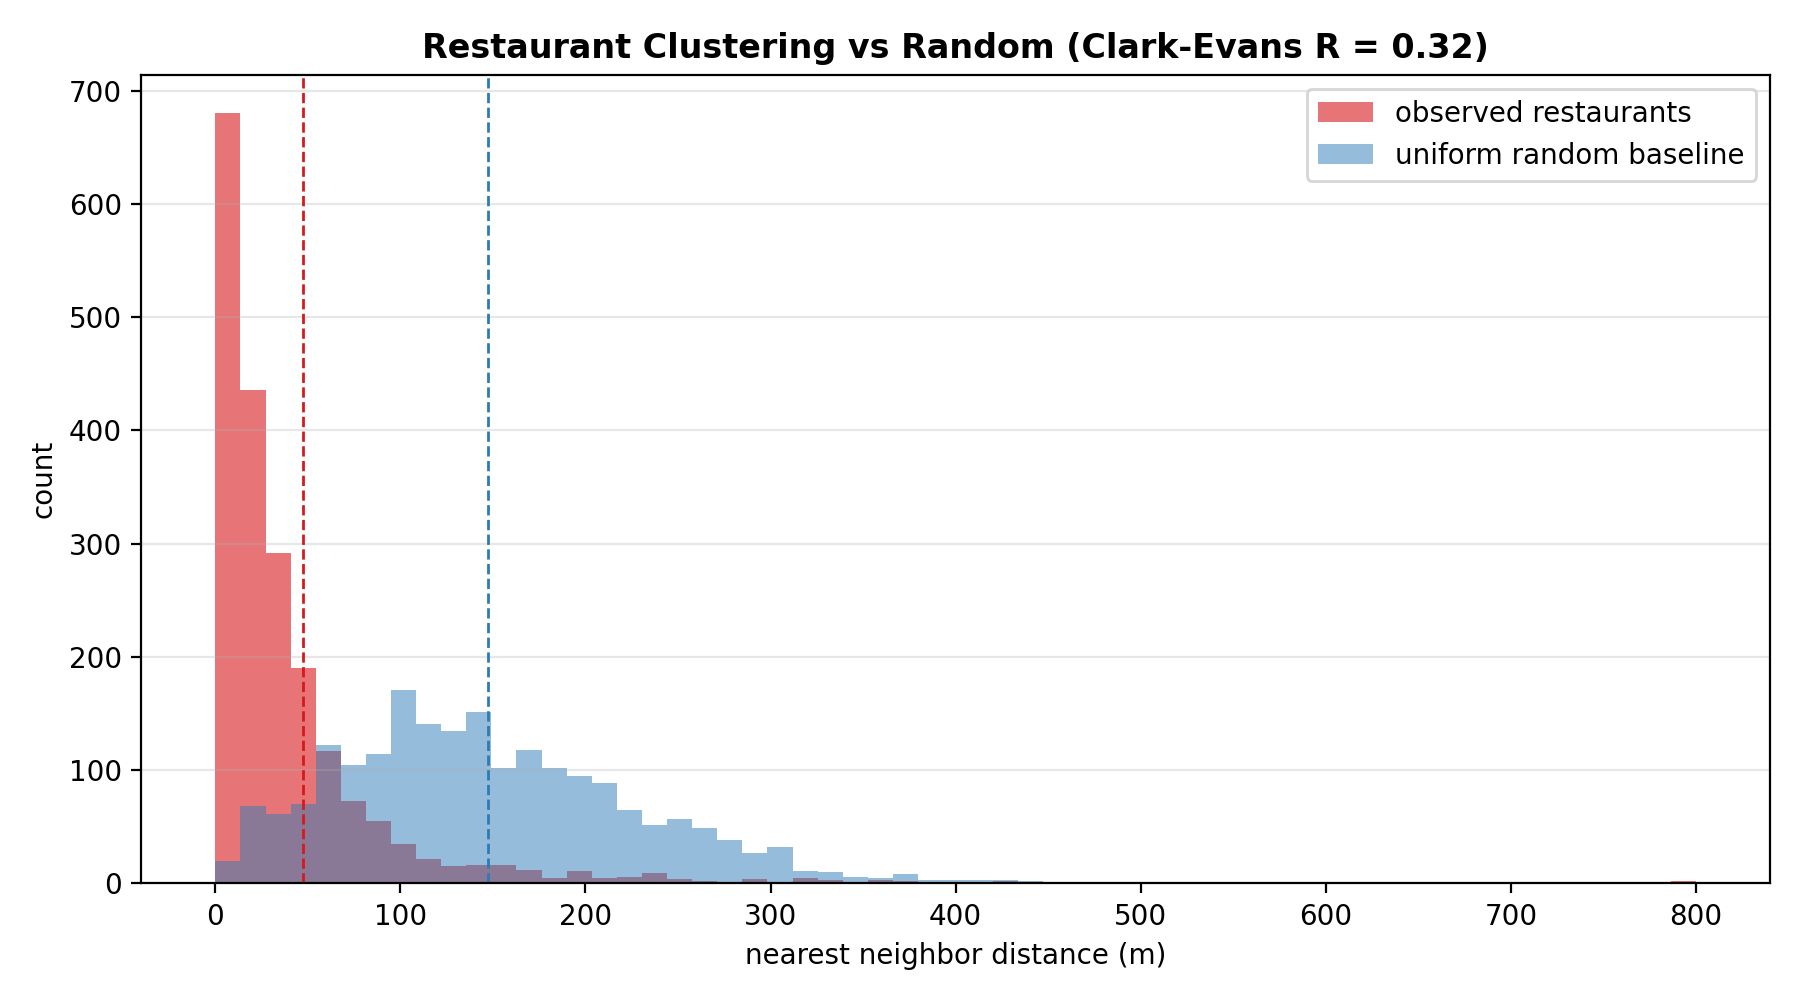
\includegraphics[width=0.85\linewidth,height=\textheight,keepaspectratio]{outputs/04_restaurant_clustering.png}

}

\caption{\label{fig-clustering}Restaurant clustering against a uniform
random baseline.}

\end{figure}%

As we can see from the plot above, the observed nearest neighbor
distances sit far to the left of the random baseline. The mean observed
spacing is 47 m against an expected 147 m under complete spatial
randomness, a Clark-Evans ratio of 0.32, which matches the clustering
behavior found in Milan by Leonardi and Moretti (2023). On the access
half, restaurants inside clusters reach the common demand sample in 8.29
minutes on average against 9.88 minutes for isolated restaurants, an
advantage of about 16 percent. Clusters sit where the street network is
fastest to everywhere else, so on static accessibility clustering helps
delivery rather than hurting it. What this comparison cannot capture is
congestion inside clusters at peak and the batching effects that Liang
et al. (2024) show matter most during rushes, so we treat the
operational half of RQ4 as open for the assignment analysis.

\phantomsection\label{refs}
\begin{CSLReferences}{1}{0}
\bibitem[\citeproctext]{ref-joshi2022}
Joshi, Manas, Arshdeep Singh, Sayan Ranu, Amitabha Bagchi, Priyank
Karia, and Puneet Kala. 2022. {``FoodMatch: Batching and Matching for
Food Delivery in Dynamic Road Networks.''} \emph{ACM Transactions on
Spatial Algorithms and Systems} 8 (1): 1--25.
\url{https://doi.org/10.1145/3494530}.

\bibitem[\citeproctext]{ref-leonardi2023}
Leonardi, Marco, and Enrico Moretti. 2023. {``The Agglomeration of Urban
Amenities: Evidence from Milan Restaurants.''} \emph{American Economic
Review: Insights} 5 (2): 141--57.
\url{https://doi.org/10.1257/aeri.20220011}.

\bibitem[\citeproctext]{ref-liang2024}
Liang, Yile, Jiuxia Zhao, Donghui Li, Jie Feng, Chen Zhang, Xuetao Ding,
Jinghua Hao, and Renqing He. 2024. {``Harvesting Efficient on-Demand
Order Pooling from Skilled Couriers: Enhancing Graph Representation
Learning for Refining Real-Time Many-to-One Assignments.''} arXiv.
\url{https://arxiv.org/abs/2406.14635}.

\bibitem[\citeproctext]{ref-reyes2018}
Reyes, Damian, Alan L. Erera, Martin Savelsbergh, Sagar Sahasrabudhe,
and Ryan O'Neil. 2018. {``The Meal Delivery Routing Problem.''}
Optimization Online.
\url{https://optimization-online.org/wp-content/uploads/2018/04/6571.pdf}.

\end{CSLReferences}




\end{document}
